\chapter{Addestrare Reti Neurali Profonde}
\begin{flushright}\small\textit{Lezione 11 -- 27/04/2026 -- G\'eron, Cap.\ 11}\end{flushright}

\section{Problemi nell'addestramento di reti profonde}

Addestrare una rete neurale profonda (DNN) con molti layer nascosti non è semplice. I problemi principali sono:

\begin{itemize}
    \item \textbf{Gradienti instabili}: i gradienti possono diventare molto piccoli (\emph{vanishing gradient}) o molto grandi (\emph{exploding gradient}) durante la backpropagation, rendendo difficoltoso l'addestramento dei layer inferiori.
    \item \textbf{Dati insufficienti}: modelli con milioni di parametri richiedono enormi quantità di dati etichettati per evitare l'overfitting.
    \item \textbf{Tempistiche di training}: l'addestramento può essere estremamente lento.
\end{itemize}
\section{Il problema del vanishing/exploding gradient}

Durante la backpropagation, l'errore viene propagato dall'output verso l'input. Spesso i gradienti diventano sempre più piccoli man mano che si procede verso i layer inferiori (\textbf{vanishing gradient}). In alcuni casi, accade il contrario: i gradienti crescono in modo esplosivo (\textbf{exploding gradient}), portando a aggiornamenti dei pesi instabili e alla divergenza dell'addestramento.

Uno dei motivi principali è la scelta della funzione di attivazione \textbf{sigmoide}, che satura per valori grandi (positivi o negativi), producendo gradienti prossimi a zero.

\begin{center}
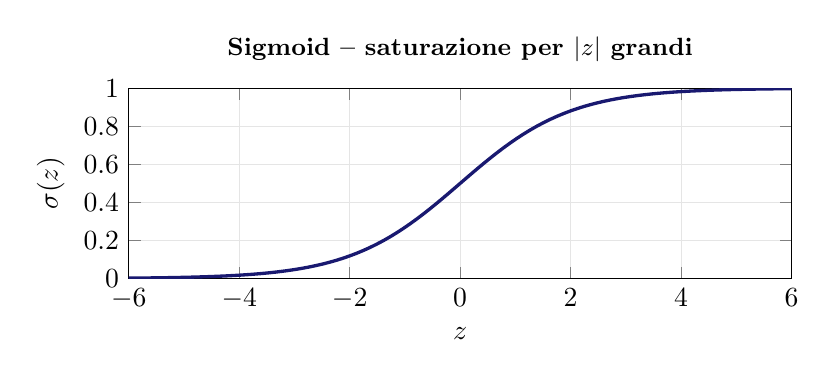
\begin{tikzpicture}
\begin{axis}[
    width=10cm, height=4cm,
    xlabel={$z$}, ylabel={$\sigma(z)$},
    xmin=-6, xmax=6, ymin=0, ymax=1,
    grid=major, grid style={gray!20},
    title={Sigmoid -- saturazione per $|z|$ grandi},
    title style={font=\small\bfseries}
]
\addplot[domain=-6:6, samples=100, very thick, MidnightBlue]
    {1/(1+exp(-x))};
\end{axis}
\end{tikzpicture}
\end{center}

\section{Inizializzazione di Glorot e He}

Una soluzione fondamentale è un'adeguata \textbf{inizializzazione dei pesi}. Glorot e Bengio (2010) proposero di inizializzare i pesi in modo che la varianza degli output di ogni layer sia uguale alla varianza dei suoi input, e lo stesso per i gradienti nella backpropagation.

\begin{defbox}[Inizializzazione di Glorot (o Xavier)]
Per le funzioni di attivazione sigmoide, tanh e softmax, si usa una distribuzione normale con varianza
\[
\sigma^2 = \frac{1}{\text{fan}_{\text{avg}}}, \qquad \text{fan}_{\text{avg}} = \frac{\text{fan}_{\text{in}} + \text{fan}_{\text{out}}}{2}
\]
o una distribuzione uniforme nell'intervallo $\left[-\sqrt{\frac{3}{\text{fan}_{\text{avg}}}}, +\sqrt{\frac{3}{\text{fan}_{\text{avg}}}}\right]$.
\end{defbox}

\begin{defbox}[Inizializzazione di He (Kaiming)]
Per ReLU e le sue varianti (Leaky ReLU, ELU, ecc.), si usa una varianza doppia:
\[
\sigma^2 = \frac{2}{\text{fan}_{\text{in}}}
\]
\end{defbox}

In Keras, è sufficiente specificare il parametro \texttt{kernel\_initializer}:
\section{Funzioni di attivazione moderne}

Le funzioni di attivazione influenzano notevolmente la stabilità dei gradienti. Ecco le più comuni:

\begin{itemize}
    \item \textbf{ReLU} ($\max(0, z)$): veloce e non satura per $z>0$, ma soffre del problema dei ``neuroni morenti'' (dying ReLU) quando l'input è sempre negativo.
    \item \textbf{Leaky ReLU} ($\max(\alpha z, z)$): introduce una piccola pendenza $\alpha$ per $z<0$ (es. 0.2), risolvendo il problema dei neuroni morenti.
    \item \textbf{ELU}: liscia e con media vicina a zero, aiuta la convergenza ma è più costosa da calcolare.
    \item \textbf{SELU}: versione scalata di ELU che auto-normalizza l'output, ma richiede condizioni specifiche (inizializzazione LeCun, input standardizzati, no dropout standard).
    \item \textbf{GELU, Swish, Mish}: funzioni moderne, lisce e non monotoniche, che spesso superano ReLU su compiti complessi.
\end{itemize}

\begin{center}
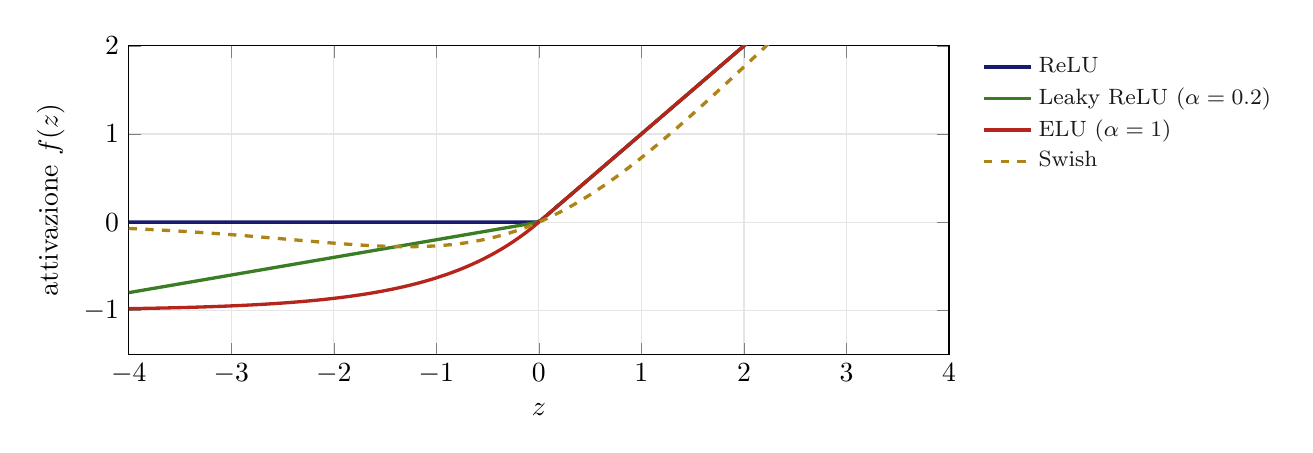
\begin{tikzpicture}
\begin{axis}[
    width=12cm, height=5.5cm,
    xlabel={$z$}, ylabel={attivazione $f(z)$},
    xmin=-4, xmax=4, ymin=-1.5, ymax=2.0,
    grid=major, grid style={gray!20},
    legend pos=outer north east,
    legend style={font=\footnotesize, cells={anchor=west},
                  legend columns=1, draw=none, fill=white, fill opacity=0.9},
    legend cell align={left}
]
\addplot[domain=-4:4, samples=200, very thick, MidnightBlue]
    {max(0,x)};
\addlegendentry{ReLU}
\addplot[domain=-4:4, samples=200, very thick, OliveGreen]
    {max(0.2*x, x)};
\addlegendentry{Leaky ReLU ($\alpha=0.2$)}
\addplot[domain=-4:4, samples=200, very thick, BrickRed]
    { (x<0) ? (exp(x)-1) : x };
\addlegendentry{ELU ($\alpha=1$)}
\addplot[domain=-4:4, samples=200, very thick, Goldenrod!80!black, dashed]
    {x * (1/(1+exp(-x)))};
\addlegendentry{Swish}
\end{axis}
\end{tikzpicture}
\end{center}

\begin{exbox}[Quale attivazione scegliere?]
\begin{itemize}
    \item \textbf{ReLU} è un buon default per compiti semplici: veloce e ben supportato.
    \item \textbf{Swish} o \textbf{GELU} sono ottimi per compiti complessi.
    \item \textbf{Leaky ReLU} è utile se si osservano molti neuroni morti.
    \item \textbf{SELU} può funzionare molto bene per MLP profondi, ma attenzione ai vincoli.
\end{itemize}
\end{exbox}

\section{Gradient Clipping}

Per il problema dell'\textbf{exploding gradient}, una soluzione efficace è il \textbf{gradient clipping}: si limitano i gradienti a un valore massimo (o norma massima) prima dell'aggiornamento dei pesi.

Questa tecnica è particolarmente utile nelle \textbf{reti ricorrenti} (RNN).

\section{Ottimizzatori: Momentum}

Lo SGD classico può essere lento. Lo \textbf{ottimizzatore con momentum} accelera la convergenza aggiungendo una frazione dell'aggiornamento precedente all'aggiornamento corrente.

\subsection{Momentum}

\begin{equation}
\begin{cases}
\mathbf{m} \leftarrow \beta \mathbf{m} - \eta \nabla_{\boldsymbol{\theta}} J(\boldsymbol{\theta}) \\
\boldsymbol{\theta} \leftarrow \boldsymbol{\theta} + \mathbf{m}
\end{cases}
\end{equation}

dove $\beta$ è il \textbf{momentum} (tipicamente 0.9). L'aggiornamento accumula velocità nelle direzioni di gradiente costante, accelerando la convergenza.

\subsection{Nesterov Accelerated Gradient (NAG)}

Una variante che calcola il gradiente non nella posizione attuale $\boldsymbol{\theta}$, ma in $\boldsymbol{\theta} + \beta \mathbf{m}$ (una ``previsione'' della prossima posizione). Questo riduce le oscillazioni e converge più velocemente.

\begin{notebox}[Adam]
Adam combina momentum e adattamento del learning rate ed è spesso il primo ottimizzatore da provare. AdamW è una variante con weight decay corretto.
\end{notebox}

\section{Tecniche di regolarizzazione per evitare overfitting}

Le reti profonde hanno molti parametri e tendono a overfittare. Ecco le tecniche principali.

\subsection{Regularizzazione $\ell_1$ e $\ell_2$}

Si aggiunge un termine di penalità alla funzione di costo:
\begin{itemize}
    \item $\ell_2$ (Ridge): $\frac{\alpha}{2} \sum \mathbf{w}^2$ (pesi piccoli)
    \item $\ell_1$ (Lasso): $\alpha \sum |\mathbf{w}|$ (pesi sparsi)
\end{itemize}

\subsection{Dropout}

Ad ogni passo di training, ogni neurone (esclusi quelli di output) ha una probabilità $p$ di essere ``droppato'' (ignorato). Questo forza la rete a non dipendere troppo da singoli neuroni, migliorando la generalizzazione. La probabilità di dropout è tipicamente tra il 10\% e il 50\%.

\begin{center}
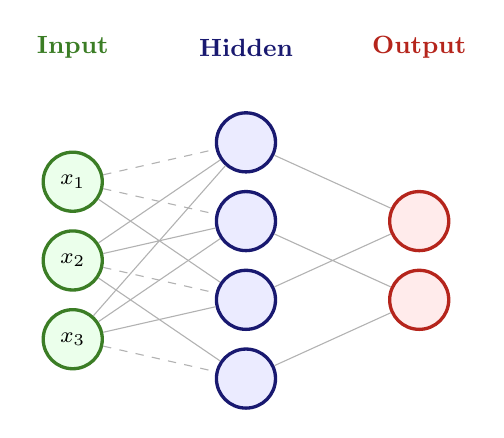
\begin{tikzpicture}[font=\footnotesize, x=2.2cm, y=1.0cm,
    inp/.style={circle, draw=OliveGreen, fill=green!8, very thick,
                minimum size=0.75cm, inner sep=0pt},
    hid/.style={circle, draw=MidnightBlue, fill=blue!8, very thick,
                minimum size=0.75cm, inner sep=0pt},
    outn/.style={circle, draw=BrickRed, fill=red!8, very thick,
                minimum size=0.75cm, inner sep=0pt}
]
\foreach \i/\lbl in {1/$x_1$, 2/$x_2$, 3/$x_3$}
    \node[inp] (i\i) at (0, -\i+0.5) {\lbl};
\foreach \j in {1,2,3,4}
    \node[hid] (h\j) at (1, -\j+1.0) {};
\foreach \k in {1,2}
    \node[outn] (o\k) at (2, -\k+0.0) {};
\draw[gray!60, thin, dashed] (i1) -- (h1) (i1) -- (h2) (i2) -- (h3) (i3) -- (h4);
\draw[gray!60, thin] (i1) -- (h3) (i2) -- (h1) (i2) -- (h2) (i2) -- (h4);
\draw[gray!60, thin] (i3) -- (h1) (i3) -- (h2) (i3) -- (h3);
\draw[gray!60, thin] (h1) -- (o1) (h2) -- (o2) (h3) -- (o1) (h4) -- (o2);
\node[font=\small\bfseries, OliveGreen] at (0, 1.2) {Input};
\node[font=\small\bfseries, MidnightBlue] at (1, 1.2) {Hidden};
\node[font=\small\bfseries, BrickRed] at (2, 1.2) {Output};
\end{tikzpicture}
\end{center}

\subsection{Max-norm regularization}

Vincola la norma $\ell_2$ dei pesi in ingresso a ogni neurone a essere $\leq r$. Dopo ogni aggiornamento, se $\|\mathbf{w}\|_2 > r$, si riscala: $\mathbf{w} \leftarrow \mathbf{w} \frac{r}{\|\mathbf{w}\|_2}$.


\begin{exbox}[Regolarizzazione: consigli pratici]
\begin{itemize}
    \item \textbf{Early stopping}: è spesso la tecnica più efficace e semplice.
    \item \textbf{Batch normalization}: regolarizza naturalmente.
    \item \textbf{Dropout}: molto efficace, specialmente per reti grandi (con tassi tra 0.2 e 0.5).
    \item \textbf{Max-norm}: utile in combinazione con dropout.
    \item \textbf{$\ell_2$}: ok con SGD, ma con Adam usare AdamW.
\end{itemize}
\end{exbox}

\section{Tecniche per reti profonde}

\begin{center}
\renewcommand{\arraystretch}{1.3}
\begin{tabular}{@{} p{3.2cm} p{5.2cm} @{}}
\toprule
\textbf{Problema} & \textbf{Tecnica} \\
\midrule
Vanishing/Exploding gradient & Glorot/He initialization, Batch Normalization, Gradient Clipping \\
Lenta convergenza & Momentum, Nesterov, Adam \\
Overfitting & Dropout, $\ell_1$/$\ell_2$ reg., Max-norm, Early Stopping \\
Scarsa generalizzazione & Data augmentation, Transfer learning \\
\bottomrule
\end{tabular}
\end{center}